 \documentclass[conference]{IEEEtran}
\IEEEoverridecommandlockouts
% The preceding line is only needed to identify funding in the first footnote. If that is unneeded, please comment it out.
\usepackage{cite}
\usepackage{amsmath,amssymb,amsfonts}
\usepackage{algorithmic}
\usepackage{graphicx}
\usepackage{textcomp}
\usepackage{xcolor}
\usepackage{url}
\def\BibTeX{{\rm B\kern-.05em{\sc i\kern-.025em b}\kern-.08em
    T\kern-.1667em\lower.7ex\hbox{E}\kern-.125emX}}
\begin{document}

\title{The role of IoT in Intelligence campus\\
%{\footnotesize \textsuperscript{*}Note: Sub-titles are not captured in Xplore and
%should not be used}
\thanks{Identify applicable funding agency here. If none, delete this.}
}

\author{\IEEEauthorblockN{1\textsuperscript{st} Andy Cui (Xiang-Yu Cui)}
\IEEEauthorblockA{\textit{Artificial Intelligence (College of Khoury)} \\ 
\textit{Northeastern University}\\
Boston, The United States \\
cui.xiangyu@northeastern.edu}
\and
\IEEEauthorblockN{2\textsuperscript{nd} Zi-yao Wu}
\IEEEauthorblockA{\textit{Electrical and Computer Engineering (College of Engineering)} \\
\textit{Northeastern University}\\
Boston, The United States \\
wu.ziya@northeastern.edu}
%\and
%\IEEEauthorblockN{3\textsuperscript{rd} Given Name Surname}
%IEEEauthorblockA{\textit{dept. name of organization (of Aff.)} \\
%\textit{name of organization (of Aff.)}\\
%City, Country \\
%email address}
%\and
%\IEEEauthorblockN{4\textsuperscript{th} Given Name Surname}
%\IEEEauthorblockA{\textit{dept. name of organization (of Aff.)} \\
%\textit{name of organization (of Aff.)}\\
%City, Country \\
%email address}
%\and
%\IEEEauthorblockN{5\textsuperscript{th} Given Name Surname}
%\IEEEauthorblockA{\textit{dept. name of organization (of Aff.)} \\
%\textit{name of organization (of Aff.)}\\
%City, Country \\
%email address}
%\and
%\IEEEauthorblockN{6\textsuperscript{th} Given Name Surname}
%\IEEEauthorblockA{\textit{dept. name of organization (of Aff.)} \\
%\textit{name of organization (of Aff.)}\\
%City, Country \\
%email address}
}

\maketitle

\begin{abstract}
As the dramatic improvement of current intelligent devices, a campus's traditional infrastructure falls behind with teachers' and students' requirements increasingly. Information constructions at colleges have transferred from digitized campus to intelligence campus. Intelligence campus is the development trend of education information construction, especially the widespread application of wireless sensors and internet things technology. The development and promotion of the internet of things, mobile learning equipment, wireless network equipment, and intelligent software have greatly improved intelligent campus applications. The technology of data and the Internet of Things help all students and faculty instructors achieve more efficient teaching and research tasks. The construction of a more efficient education ecosystem aims to explore wireless sensors and internet things technology in innovative campuses and propose a development strategy from smart campus to efficient intelligence campus construction.


\end{abstract} 

\begin{IEEEkeywords}
Intelligence Campus, Wireless Sensor, Big Data, Artificial Intelligence, Internet of Things
\end{IEEEkeywords}

\section{Introduction}
The global Internet of Things (IoT) moves from the initial stage of fragmentation and independent application into a new phase of "focus, crossover integration, and integrated innovation." With the rapid start of the market and accelerated penetration in many fields, the Internet of Things is on the eve of leapfrog growth \cite{INTCAMPUS:ResearchOnApp}. Due to COVID-19, all departments of education accelerated the pace for digital education. An intelligent college campus is character interconnection, intelligence, interaction, mobility, openness, and sharing. It mainly has three core functions: Firstly, it provides a comprehensive intelligent sensing environment and comprehensive information service platform for teachers and students, and provides personalization and customization service based on role; Second, integrate the information service based on computer network into each application and service field of the school to realize interconnection and collaboration; The third is to provide an interface for mutual communication and perception between the school and the outside world through the intelligent perception environment and integrated information service platform \cite{INTCAMPUS:TechDevelop}. 

American educator Dewey proposed in "Schools and Society":  "Schools and Society, which is the reform of  the education system must be affected by the profound progress of social progress \cite{INTCAMPUS:AnalysisApplication}." In short, like an intelligent mini-city, an intelligent campus leverages devices and apps to create new experiences or services and promote operational efficiency. Smart campuses will be the prototype of smart cities and are easier to implement because they have clear ownership and limited goals. Smart campuses linked to office space, service and retail centers, and educational institutions have begun their journey towards becoming technology hubs using new technologies \cite{INTCAMPUS:AppOfAI}. 

Innovative campus needs to introduce artificial intelligence and big data in the direction of the Internet of Things and data architecture and apply low-energy technologies. The networked classroom, the smart classroom, is also a vital link. Various elements in the innovative classroom environment build a modern learning environment foundation for blended learning online and offline to improve to promote modern education continuously \cite{INTCAMPUS:AppofIntClass}. At present, the blended learning model is widely applied in the current offline teaching. Such teaching mode has the fun and richness of online learning and has the standardization of offline education, so this kind of education mode is prevalent. We will discuss all existing structures of intelligent campus and improve parts in our survey paper. The paper will include IoT Based Framework for Implementation, Low Power Wide Area Internet of Things in College Smart Campus, IoT for Intelligence Campus future improvement. 

\section{IoT Based Framework for Implementation}

\subsection{Intelligence Campus Focus Areas}

Intelligence campuses provide convenient and efficient services to students and faculty. In short, smart campuses will provide a rapid return on investment to stakeholders. The focus is on operational efficiencies, such as energy-saving, reduced downtime, and end-user comfort, utility, and experience.  According to the P. Agarwal (2020) report, they divided the implementation across three broad areas which need to have the sustained focus to achieve the intelligent campus operational efficiencies and functionalities: Sustainability, Infrastructure, End-user utility, and experience \cite{INTCAMPUS:IoTbasedFrame}.

\begin{itemize}
\item Sustainability  Focus:  Sustainability  is  one  of  the  key  focus  areas for organization, key focus areas being:  
\begin{itemize}
%            \setlength{\itemindent}{-.2in}
            
  \item Energy:  Focus  on  reducing  energy  consumption,  increasing  energy  efficiency,  Green  Computing  and  use renewable energy sources to lower greenhouse gas (GHG) impact.  
  \item Water:    Focus  on  campuses  water  sustainable  and  continue to reduce per capita freshwater consumption 
  \item Waste Management: Structured approach to manage different kinds of  generated waste 
  \item Emissions: Reducing the Green House gas emissions, target to become carbon neutral.
\end{itemize} 
\item Infrastructure Focus: Focus on Building smart infrastructure and   implementing   the   use   cases   which   helps   in   smart   Infrastructure
  \begin{itemize}
  \item Data Centers for catering to IT needs 
  \item Cloud based infrastructure 
  \item Building Management Systems 
  \item Unified Communication system 
  \item Smart Parking - Automated 
  \item Automated Transport  
  \item Installation of Sensors and measuring right parameters
  \end{itemize}
  
 
  
\item End  User  Utility  and  Experience:    Enhancing  the  user  experience leveraging the data captured from various end points and developing the applications to enhance the user experience in the campus. These use cases are evolving and some of these examples are:
\begin{itemize}
  \item Smart Cafeteria 
  \item Health and Wellness App 
  \item Intelligent Access control  
  \item Smart Indoor Navigation 
  \item Visitor Management 
  \item Safety and Security related applications 
  \item Room Booking 
  \item Smart Occupancy, Dynamic Seat Allocation

\end{itemize}
\end{itemize}
\subsection{Five  layered  IoT  Framework  to  realize  Smart  Campus Vision}


We know about the leading five-layered IoT Framework of Smart campus, as we showed from the current article source. For intelligent campus construction development, several sensors and other IoT devices are needed to gather the information together. Edge nodes, aggregators, data servers, and other devices are required to connect smart campus devices to IoT systems. The sensor generates information at high speed, which requires a Hadoop system to achieve \cite{INTCAMPUS:ANovelFrame}. According to the requirements and constraints of wireless sensor networks and the Internet of Things, Hossain's team design a good Intelligence campus working module in 2019. They designed the working model for our proposed IoT-based different application services. Conceptual working models for innovative environment monitoring systems, intelligent car parking systems, and intelligent canteen management systems are illustrated in Fig. 3(a), 3(b), and 3 (c), respectively \cite{INTCAMPUS:FlexibleTech}. 

\begin{wrapfigure}{Figure}{.1 Structure of Intelligence Campus Big Data Analytics\textwidth} %this figure will be at the left
    
    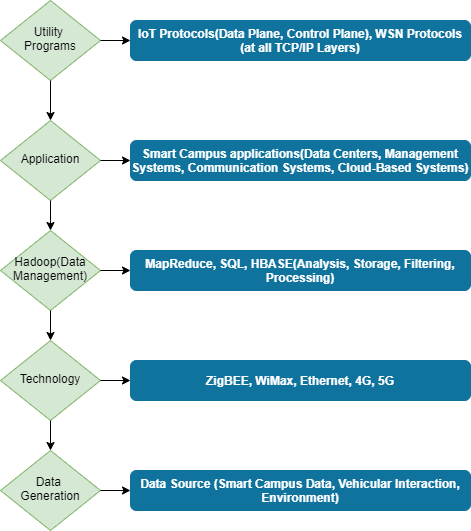
\includegraphics[width=8.4cm, height=12cm\textwidth]{bibliography/images/diagram1new.png}
\end{wrapfigure}
%----------------------------------------------------------------------------



%----------------------------------------------------------------------------
The sensor and Data Acquisition layer will capture the data leveraging various sensors on a real-time basis and will send it to upper layers for processing. 

Compute and Infrastructure layer will provide the required infrastructure to store the data and connecting with data sensor and data acquisition layer using various network connectivity methods. It includes connecting the required gateways, devices, and sensors such as Wi-Fi, BLE, ZigBee \cite{INTCAMPUS:IOTBasedModel}. 

The platform layer will help create the unified layer, which will help communicate with various heterogeneous systems catering to the same or distributed functionalities. It will help integrate and collect the data from existing and new systems and take care of security requirements.

Application Layer will help define implementing the use cases, which will help realize an intelligent campus's objective. The acquired data will be available from the platform layer on a real-time basis, and the use cases can be implemented on top of this.

The monitoring layer will monitor the applications and generate the required alerts and interventions based on need. Command Center or dashboards can be set up based on applications that need to be monitored regularly.

\subsection{Intelligence Campus Working Modules}
The team of Hossain designed a good Intelligence campus working module in 2019. They designed the working model for our proposed IoT-based different application services. Conceptual working models for an innovative environment monitoring system, an intelligent car parking system, and an intelligent canteen management system are illustrated in Fig. 2 (a), 3(b), and 3 (c), respectively\cite{INTCAMPUS:IOTBasedModel}. 
%三张图放在这里



\begin{wrapfigure}
    \centering
    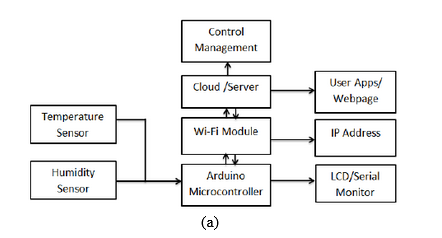
\includegraphics[width=0.5\textwidth]{bibliography/images/a.png}
\end{wrapfigure}

\begin{wrapfigure} 
    \centering
    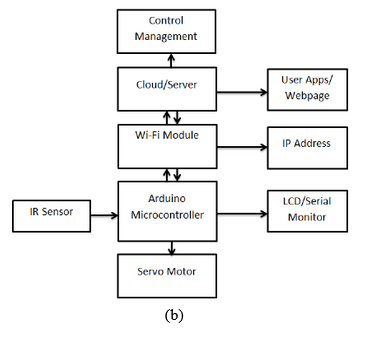
\includegraphics[width=0.5\textwidth]{bibliography/images/b.png}
\end{wrapfigure}

\begin{wrapfigure}
    \centering
    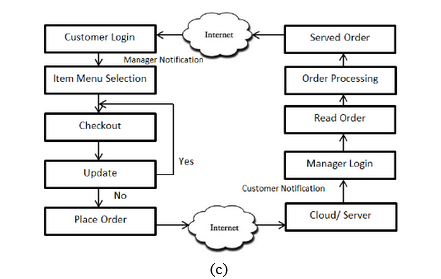
\includegraphics[width=0.5\textwidth]{bibliography/images/c.png}
\end{wrapfigure}

Figure.2(a),(b),(c)
Conceptual working model of (a) smart environment monitoring system, (b) smart car parking system, (c) smart canteen system. 

\subsection{Intelligence Campus Implementation – Case Studies}
In the 1970s, the Massachusetts Institute of Technology (MIT) in the United States first proposed Electronic Campus. In 1990, Professor Kenneth of Claremont University put forward the concept of Digital Campus for the first time and led the Campus Computing Project (CCP) scientific research Project. Since the CCP plan, the U.S. government successively in 1996 and 2000, 2005, 2010, promulgated and implemented a national plan: education technology scheme and university implementation. The object is man, machine, road, mesh piece junction, revolutionized the American higher education mode with the combination of teaching and learning, means and process, to make America's education informationization in the leading international position. The United States has always followed the strategic principle of "information technology to promote education reform and development," experienced a reform process from "infrastructure construction - system application - operation effect - structural adjustment," and gradually transformed from electronic campus to digital campus and innovative campus. Many Countries such as Britain, Australia, New Zealand, and Japan also developed and implemented education promotion projects. The United Kingdom has issued a series of plans named forward education highway plan and 2010-2012 education development strategy; Australia introduced a digital education revolution implementation roadmap; New Zealand set a school digital learning action plan; Japan implemented the school network plan. These action plans and strategies provide exemplary examples and experiences for other countries to transition from digital to intelligent campuses. We have seen the focus on intelligent campus implementation worldwide to achieve sustainability and enhance the user experience. \\

\textbf{Smart Campus implementation for leading companies & universities:} \\

Google \cite{INTCAMPUS:GoogleReport} has focused on sustainable workplaces, saving 40,000 tons of carbon dioxide emissions and preventing 6.6 million pounds of food waste using the Google shuttle in the Bay Area. There are 13 million square feet of green building LEED-certified workspaces focused on sustainable workplaces. For the second year in a row, 100\% of the electricity needed for global operations comes from renewable sources. \\

Microsoft \cite{INTCAMPUS:MicrosoftReport} announced to modernize the Redmond campus (Microsoft headquarters). Microsoft is modernizing its workplace to make it an intelligent campus and use its campus as an innovative living laboratory that focuses on the campus and community and enhances the employee experience. \\ 

Amazon \cite{INTCAMPUS:AmazonReport} company offices in Seattle focuses on sustainability, energy conservation, and responsible use of resources. They built a 40K houseplant greenhouse on their Seattle campus that provides a natural source of insulation and cooling. They focus on sustainable design and experience in their upcoming campus. The United States Green Building Council has awarded LEED (Leadership in Energy and Environmental Design) certification to 26 buildings in Seattle. \\

Infosys \cite{INTCAMPUS:InfosysReport}, a leading IT service provider in India, has over 25 million LEED-certified offices. Their campus is a living laboratory for clean technology applications, focusing on sustainability and improving the employee experience. From 2008 to 2019, per capita, energy consumption declined by 55\%, with 44.3\% of electricity consumption coming from renewable energy sources. The Carbon Offset PortPortio and the Carbon Neutral Journey have won the 2019 UN Global Climate Action Award.  \\

Arizona State University \cite{INTCAMPUS:ArizonaBuiltCampus}, a top university in the United States, uses the Internet of Things and the next generation of technology to achieve an intelligent campus. Implementing new use cases to make it an intelligent campus, coupled with its innovation focus, is ongoing. For example, they have a connected stadium that uses real-time data from sensors to enhance the fan experience. \\


\subsection{EXTENDING NEW USE CASES FOR IOT BASED FRAMEWORK}

Agarwal's team (2020) implemented use cases related to COVID-19 to safeguard employee health, and they tried the five-tier framework described in Table-1 to implement the Smart Campus case.
%---------------------------Table-1 ----------------------------
\begin{wrapfigure}
    \centering
    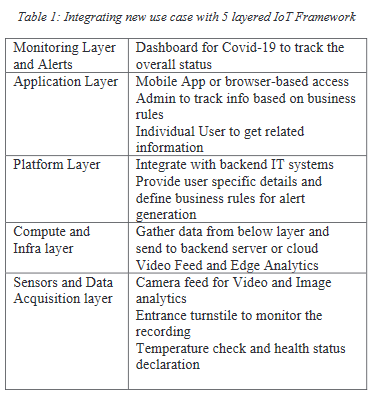
\includegraphics[width=0.5\textwidth]{bibliography/images/Table-1.png}
\end{wrapfigure}
%-------------------------------------------------------------------
The COVID-19 use case will need to identify the appropriate sensors, hardware, technology stack, and it has to be defined in conjunction with IT systems and integration requirements \cite{INTCAMPUS:ApplicationOfSmartCity}.

\section{Low Power Wide Area Internet of Things in College Smart Campus}
\subsection{Application of low power wide area network in university teaching and research management}
 
Traditional wired or wireless Internet of Things technologies, such as RFID, have been applied in many conventional scenarios, such as classroom attendance, library staff entry, exit, book management, teaching buildings, laboratory access control, etc. These schemes are relatively mature with low cost, but they need to punch manually. Sometimes, it is easy to forget to punch, and it is impossible to recognize the entry and exit of the classroom in real-time after punching. Low-power-wan technology can be introduced to ring or too class RFID electronic label detectors, transform the traditional RFID probe into RFID + low-power wan technology products, both in and out of the classroom through the door every time new detector automatic identification and implement wireless remote transmission of data, this can improve the efficiency of management and increase the teaching class real-time dynamic data collection and analysis. For example, it optimizes classroom discipline, counting the attendance rate and the popularity of some public elective courses, providing closed-loop feedback to teaching, and helping teachers and the academic affairs office improve teaching quality and reform teaching. RFID scheme can also extend to the staff entry and exit of the library and the book management. It can count the library's staff entry and exit and monitor and remind the unregistered books taken out of the library by mistake in real-time. 

Low-power wide-area IoT can be used for asset inventory and asset entry and exit management in university warehouses or laboratories. Many university laboratories still use manual methods for asset inventory and control, which is inefficient and difficult to stock. With the introduction of low-power WAN technology, the RFID tag technology can be attached to each asset and device. In contrast, RFID+ low-power WAN technology detectors can fix at the entrance and exit of the laboratory. In this way, the assets entering and leaving the laboratory each time will automatically detect by the fixed detector and reported to the system in real-time, facilitating the automatic real-time management of assets entering and leaving. Portable detectors can use for periodic asset inventory. Instruments are often borrowed between different university laboratories, especially unregistered ones, which will cause difficulties in searching for regular inventory. Using mobile detectors for a circle can capture asset information within a range close to one meter, thus improving inventory counting efficiency.

Low-power wide-area Internet of Things technology can also be applied to the process of scientific research experiments. Through voltage, current, or vibration sensors, real-time data detection can carry out to automatically judge whether the investigation is interrupted and send out an alarm to timely detect and intervene in the recovery. Low-power wide-area Internet of Things technology can also help realize the remote acquisition of experimental data and the remote sensing of instructions to adjust the practical scheme to improve the experiment's efficiency and security. Besides, low-power wide-area IoT technology has many other application scenarios and values, such as abnormal temperature detection of products or equipment in the laboratory process, abnormal movement alarm of experimental instruments or essential assets, environmental temperature and humidity monitoring, real-time detection, and notice of flammable, explosive or toxic gases, etc.\cite{INTCAMPUS:BriefAnalysis}


\subsection{Application of low power wide area network in campus life and security management}

The Internet of Things technology can realize real-time observation and monitoring of the campus's surrounding environment and effectively eliminate all kinds of unstable factors \cite{INTCAMPUS:AppAndDevOfIOT}. In the application of the Internet of Things in college campus life, the traditional wired or wireless Internet of Things technology, such as RFID, has realized the general consumer applications in places such as dormitories, dining halls, supermarkets, bathrooms, teaching buildings, and public campus areas, which can meet the needs of actual operation, and the solutions are relatively mature and popular. However, in the application of energy management in college campus life, the low power wide area Internet of Things technology has its unique advantages. For example, the low power wide-area Internet of things technology apply to the university interior lighting, especially corridor lighting and outdoor street light in the scene on campus, can take advantage of the light environment, sound sensor, automatic linkage to the relevant electrical control of lighting equipment or dimmer module, realizes the remote lighting switch, dimmer, fault monitoring alarm and power consumption data collection. Due to the low power consumption of such low-power, wide-area technology Internet of Things sensors, they can be deployed wirelessly using battery power.
In most cases, sensor modules can install existing lighting facilities without repeating the existing facilities' construction. The scheme deployment is simple, remote monitoring and maintenance are convenient, and the total cost is low. Many indoor areas, such as teaching buildings, laboratories, libraries, dormitories, canteens, etc. Facilities equipped with air conditioners often resulting in energy waste caused by forgetting to turn off the air conditioners or unreasonable air conditioning temperature settings. By introducing a low-power wide-area Internet of things technology, equipped with corresponding indoors actual indoor temperature for real-time monitoring of temperature sensor and wireless remote transmission to the management platform, combined platform area received video or infrared monitoring data to determine, can realize the air conditioning forget to closed management and temperature setting reasonable management, avoid waste of energy.

In college campus security management, in addition to typical RFID access control applications and 3G/4G service-based video security monitoring applications, vehicle and parking space management workload is enormous and complex; once the management is not timely or not in place, it will also cause security accidents. So people can enter the campus of bikes and cars in IoT electronic tags based on the technology of low power wan card, with its low power consumption, long-distance transmission, and scale of the characteristics of the network application, on the one hand, can be in and out of campus identification and frequency statistics. On the other hand, it can combine positioning technology for all kinds of vehicle positioning management queries and disorderly parking place management and maintain campus management and order. Besides, it can also achieve exemplary leadership, set up electronic fences, some areas in the campus do not allow motor vehicles to enter, be real-time monitoring and management, and improve campus safety management \cite{INTCAMPUS:ResearchOnWideCoverage}.

Indoor safety management of IoT can realize installing smoke sensors, open fire sensors, and flood sensors in university buildings. It can also send alarm signals and when emergency facilities can be started after parameters exceed the standard, effectively reducing disasters. Compared with the traditional wired scheme, such sensors' battery-powered method based on the low-power wide-area Internet of Things technology is more convenient and efficient to deploy. The signal stability and long transmission distance can improve the real-time and effectiveness of alarms \cite{INTCAMPUS:AppofIOTinSmartCampus}. The management of some security doors or particular areas often closed doors in colleges and universities requires that there can be no open and exit in the normal state for a long time. Once there is an abnormal available, it is necessary to alarm in time and notify relevant personnel to view the scene. Go through the help of a battery-powered and low-power WAN wireless door magnetic sensor, and the security system applications can be deployed.

\subsection{Application of Wide Area Internet of Things in Predictive Maintenance of Campus Equipment}

There are many essential equipment and facilities of campus that need to work generally in an extended period. When some fault or abnormal kits appear, it could lead to many security problems and economic losses. For instance, we might suffer air conditioning outside machine failure, distribution transformer faults, water pump failure, harmful gas emissions fan fault, significant scientific instruments equipment failure, abnormal pressure water or gas lines, and so on \cite{INTCAMPUS:SDN-BasedIOT}. So, when we import IoT and AI technologies to monitor and maintain these systems, the edge of the calculation of artificial intelligence technology combined with intelligent predictive maintenance sensors will distinctly, which indicates that low power consumption, long transmission distance, and simple deployment, remote maintenance convenient. These intelligence devices can significantly improve the intellectual level of local processing and response speed, reduce labor costs, and reduce equipment failure caused by safety accidents, property damage, and maintenance cost. Thus, IoT and AI devices further enhance the intelligent campus construction effect and level's comprehensive management.

\section{IoT for Intelligence Campus future improvement}
We learned two significant Intelligence Campus fields, which are IoT Based Framework for Implementation and Low Power Wide Area Internet of Things in College Smart Campus. Our topic is The role of IoT in the Intelligence campus, and we want to use IoT technology to build a digital lifestyle; that's is to say, we can use our belongings (currently is a smartphone) to help us control many required electronic equipment. Since COVID-19, all universities and educational institutes are focused on network intelligence healthy campus construction. So, the campus smart facilities need to satisfy online educational activities and in-person activities synchronously. We found that the Intelligence campus wants to supply all kinds of end-users to solve the cross-demand problems. The simple question is that different roles demand different functions. Currently, there is no denying that ensure students back to campus join in-person lecture is an urgent task. All campuses deployed Intelligence medical system. An innovative wireless network thing is that students can have a particular health ID in their phone App, and it holds their vaccination status and event venues in the last thirty days. Also, suppose the student gets the emergency. In that case, they can get the better method from his/her phone notification, such as he or she can transfer to the school medical canter or the nearest hospital, based on the data center's judgment. Otherwise, the school's medical department can disinfect and treat patients' recent activities. In terms of offline students, the campus can consider supply education special network channels to help the international student solve a live online course. 

Low energy consumption is a more significant issue of building an intelligent campus. We did a paper survey for energy issue, and we think the embedded products seems a promising direction of development. Since the team of Hossain design a good Intelligence campus working module for a bright environment monitoring system, which is an intelligent car parking system and intelligent canteen system, they use a divide and conquer algorithm to use cloud centralized data processing. Further more, Big data and artificial intelligence will develop more low-energy IoT architecture models in the future. 

\section{Conclusions}
After our investigation, we believe that IoT will help humans build an efficient and convenient living environment. However, the intelligence campus construction is a complicated, intricate system project; therefore, its structure needs a scientific and reasonable top-level design from the government and education sectors.

The intelligence campus requires the active participation of other parts of the society.  A shared intelligence campus governance system with overall government planning, school practice, and social support should establish. The quality and level of its construction can be improved and developed gently. When the graduates end their studies in their field, the governments and communities will get these students' timelines and essential information from the schools' public database. If smart campuses have popularized worldwide, the universities' employment rate will be significantly increased. There are still exist new fields, and with the advancement of IoT technology will occur many new requirements.

The construction of intelligent colleges and universities provides campus administrators with the dynamic control of teachers and students, creates a comfortable campus environment, provides convenient conditions for office work, provides assistance for students' learning, and comprehensively improves the school's governance level. In the future, new artificial intelligence and technology will continue to design more solutions and high-quality products around the campus scene and build a more advanced and scientific campus environment.

%-------------------Reference --------------------------------------------------------------------------





\bibliographystyle{./bibliography/IEEEtran}
\bibliography{./bibliography/IEEEabrv,./bibliography/IEEEexample}

\vspace{12pt}


\end{document}
